\section{Elaboración.}

La elaboración de un mapa mental es un gesto sencillo y casi intuitivo, sólo necesitamos partir de una idea central, de la cual vamos ramificando, asociando o interconectando símbolos, palabras, tareas o dibujos. 

\begin{figure}[htbp]
\centering
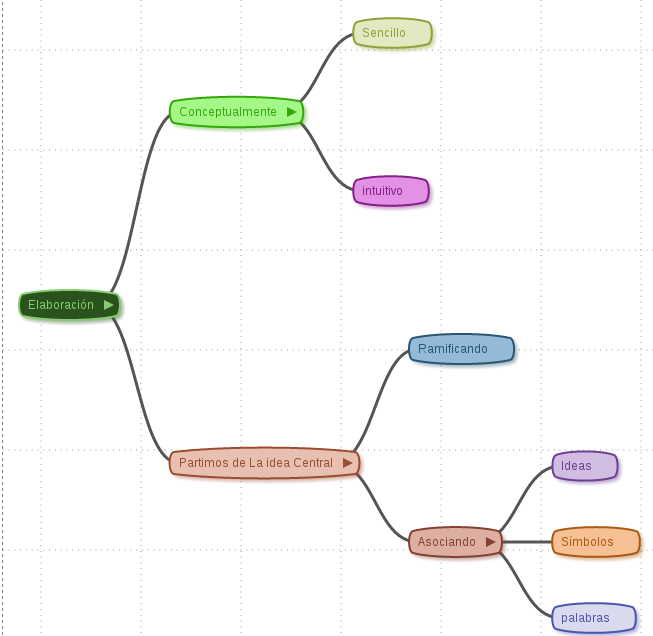
\includegraphics[width=0.7\textwidth]{imagenes/Elaboracion.png}
\caption{Mapa mental de elaboración de mapas mentales}
\label{fig:elaboracion}
\end{figure}

En definitiva, se trata de un diagrama radial que permite a una persona, o grupo de ellas,  plasmar su percepción sobre un tema, o idea, mediante la asociación de conceptos palabras y/o imágenes.

